\documentclass[12pt, a4paper]{article}
\usepackage[spanish]{babel}             % Español para los nombres
\usepackage[utf8]{inputenc}             % Codificación de entrada
\usepackage[T1]{fontenc}                % Codificación de fuente (escribir castellano)
\usepackage{lmodern}                    % Fuente (la default no es compatible con castellano)
\usepackage{csquotes}                   % Para comillas y otras anotaciones del castellano
\usepackage{fancyhdr}                   % Encabezado y Pie de pagina
\usepackage{tocloft}                    % Puntos en los índices

\usepackage{hyperref}                   % Links y referencias dentro del texto
\usepackage{acronym}                    % Para incluir las listas de abreviaturas
\usepackage{multicol}                   % Permite crear espacios con columnas verticales
\usepackage{parskip}                    % Eliminar sangrado y añadir espacio entre párrafos

\usepackage{graphicx}                   % Para incluir imágenes
\usepackage{subcaption}                 % Subfiguras
\usepackage{xcolor}                     % Definir y utilizar colores
\usepackage{tikz}                       % Dibujar formas, figuras, rectas, intersecciones...
\usepackage[absolute,overlay]{textpos}  % Posición absoluta para textos
\usepackage{geometry}                   % Para controlar los márgenes

\usepackage{float}


\usepackage[backend=biber, sorting=none]{biblatex} % Referencias (bibliografía / webgrafía)
\selectlanguage{spanish}                % Seleccionar español
\bibliography{referencias}              % Incluir el archivo de referencias

% Definición de nombres
%\printbibliography[title={Bibliografía}]
\renewcommand{\cftsecleader}{\cftdotfill{\cftdotsep}} 
\renewcommand{\spanishtablename}{Tabla}
\renewcommand{\spanishlisttablename}{Índice de tablas}
\newcommand{\estudiante}{Aróstegui García, Alberto}
\newcommand{\director}{Egaña Aranguren, Mikel; López Novoa, Unai}
\newcommand{\grado}{INGENIERÍA INFORMÁTICA DE GESTIÓN Y SISTEMAS DE INFORMACIÓN}
\newcommand{\titulo}{KG RAG}
\newcommand{\portada}{images/protada.png}
\newcommand{\curso}{2023-2024}

% Definición de Macros
\newcommand{\aclink}[1]{\hyperlink{acro:#1}{\ac{#1}}} % Enlazar la abreviatura al acrónimo

% Encabezado y Pie de pagina
\pagestyle{fancy}                       % Estilo de las páginas
\fancyhf{}
\fancyhead[L]{Trabajo Fin de Grado}
\fancyhead[R]{\rightmark}
\fancyfoot[L]{UPV/EHU}
\fancyfoot[R]{\thepage}
\renewcommand{\footrulewidth}{0.4pt} % Línea horizontal en el pie de página
\setlength{\headheight}{15.5pt}

% Definición de colores
\definecolor{ehu_blue}{HTML}{376092}
\definecolor{link_color}{HTML}{36AEB4}
\definecolor{reference_color}{HTML}{0F3133}

% Configuración de hyperref para diferentes tipos de enlaces
\hypersetup{
    colorlinks=true,
    linkcolor=reference_color,
    citecolor=reference_color,
    filecolor=link_color,
    urlcolor=link_color,
}

% #########################################################################
% #                                  TFG                                  #
% #########################################################################
\begin{document}
\newgeometry{bottom=2cm}

\begin{titlepage}
    % Logo de la universidad
    \begin{textblock*}{\textwidth}(10cm,0cm)
        
\includegraphics[width=7.5cm, height=3cm]{images/logos/Logo_EHU.jpg}
    \end{textblock*}
    
    % Franja azul
    \begin{tikzpicture}[remember picture, overlay]
        \fill[ehu_blue] (current page.north west) ++ (0,-3.01cm) rectangle (\paperwidth,-3cm);
    \end{tikzpicture}
    
    \begin{textblock*}{\paperwidth}(\dimexpr\parindent+\oddsidemargin+3em\relax,3.5cm)
        \begin{minipage}{\dimexpr\linewidth-7.5cm\relax}
            \color{white}
            \noindent\rule{\linewidth}{0cm}
            \textsf{ {\large GRADO EN \grado}}
            \newline
            \newline \newline
            \textsf{\textbf{ {\Huge TRABAJO FIN DE GRADO }}}
        \end{minipage}
    \end{textblock*}
    
    % Título del trabajo
    \vspace*{3.5cm}
    \begin{minipage}{\linewidth}
        \setlength{\baselineskip}{1.7\baselineskip}
        \centering
        \textsf{ \textbf{ {\LARGE \titulo }}}
    \end{minipage}

    % Foto de portada
    \vspace*{0.5cm}
    \begin{figure}[H]
        \centering
        
    \end{figure}

    % ODS
    \vspace*{1cm}
    \begin{figure}[h]
    \centering
        \begin{subfigure}[b]{0.135\textwidth}
            
\includegraphics[width=2cm, height=2cm]{images/iconos_ods/09.png}
        \end{subfigure}
        
        \label{fig:ods-iconos}
    \end{figure}
    
    % Estudiante
    \vspace{0.2cm}
    \noindent {\footnotesize \textbf{Estudiante:} \estudiante}
    \newline
    \noindent\makebox[\linewidth]{\rule{\textwidth}{0.4pt}} % Línea horizontal

    % Director
    \nopagebreak
    \vspace{0.3cm}
    \nopagebreak
    \noindent {\footnotesize \textbf{Director/Directora:} \director }

    % Espacio para firmas
    \vspace{0.5cm} % Espacio entre texto "Director/Directora" y espacio para firmas
    \noindent 
    \makebox[0.4\linewidth]{\hrulefill}
    \hspace{0.2\linewidth}
    \makebox[0.4\linewidth]{\hrulefill}

    % Curso y Fecha
    \vspace{0.1cm}    
    \noindent {\footnotesize \textbf{Curso: } \curso \hfill \textbf{Fecha:} \today }
\end{titlepage}

\restoregeometry
\setcounter{figure}{0} % Incluimos el título
\newpage
\begin{itshape}
    \textbf{Resumen:} \\
    Este trabajo se enfoca en explorar los límites de los ensayos a tracción para probetas de materiales compuestos.

    
    \textbf{Palabras Clave:} Materiales Compuestos
\end{itshape}
\newpage

\begin{itshape}
    \textbf{Abstract:} \\
    English


    \textbf{Key Words:}
\end{itshape}
\newpage

\begin{itshape}
    \textbf{Laburpena:} \\
    Euskera

    
    \textbf{Gako-hitzak:}
\end{itshape}
\newpage
 % Incluimos el resumen tri-lingüe

% Índices
\tableofcontents\thispagestyle{empty}\newpage
\listoffigures\thispagestyle{empty}\newpage
\listoftables\thispagestyle{empty}\newpage

% Abreviaturas
\addcontentsline{toc}{section}{Abreviaturas}
\section*{Abreviaturas}
%\begin{multicols}{2} % Si se quieren en dos columnas verticales
\begin{acronym}[ASSI]  % El acrónimo más largo
    \acro{API}{Application Programming Interface}
    \acro{JQL}{Jira Query Language}
    \acro{LLM}{Large Language Model}
    \acro{RAG}{Retrieval Augmented Generation}
    \acro{PLN}{Procesamiento del Lenguaje Natural}
\end{acronym}
%\end{multicols}

 % Marcar como visto (No te desglosa el acrónimo)
 % Provoca warnings pero funciona :)
%\acused{ADN}
%\acused{USB}
\newpage

\section{Introducción}
En 1983 el autor James Watson descubrió el \aclink{ADN} \cite{watson53}. La <<medicina>> realmente era veneno. El \aclink{ASSI} es el encargado de mostrar en todo momento el estado del \aclink{AS}. Si el \aclink{ASSI} se apaga de forma inesperada, se considerará un estado de emergencia eléctrico.
El \aclink{USB} es un protocolo de comunicación basado en el protocolo RS232.

En la wikipedia de LaTex \cite{latex_wikibook} puedes encontrar información muy útil para tus documentos.

\subsection{Estudio demográfico}
En los últimos años, la población mundial ha ido decayendo considerablemente. Tanto es así, que los países más desarrollados, los cuales son a su vez los más envejecidos, están teniendo muchas dificultades para mantener sus sistemas de pensiones. Estos hechos se ven reforzados por los datos del gráfico \ref{fig:envejecimiento} en el que se comparan distintas poblaciones Europeas \footnote{Aguacate con salami}.

\section{Contexto}

Este trabajo de fin de grado responde a las necesidades de la empresa LKS Next-GobTech\footnote{https://www.lksnext.com/es/servicios/tecnologia/gobtech/outsourcing-it-estrategico-con-lks-next/}, una empresa de desarrollo de software con enfoque en la innovación. LKS Next-GobTech es una empresa que desarrolla software a medida para sus clientes, principalmente la adminstración pública del País Vasco y, en menor medida, empresas privadas. Utilizan técnicas de desarrollo ágil y metodologías de gestión de proyectos para llevar a cabo sus proyectos.

Para comprender las necesidades de la empresa que este trabajo pretende solucionar, primero se han de poner en contexto las herramientas y metodologías que utilizan. Partiendo del TFG de un compañero de escuela, Joel García Escribano~\cite{jiragpt}, que consiste en un asistente conversacional que genera consultas JQL a partir de preguntas hechas con lenguaje natural y cuyo objetivo era dar una visión de las posibilidades de los LLMs en el desarrollo de software y proporcionar a LKS una herramienta para el futuro desarrollo de sus proyectos, se ha estudiado la posibilidad de añadir una arquitectura de RAG (Retieval Augmented Generation) para aumentar la precisión de las respuestas que ofrece.

A continuación, se detallan las herramientas y metodologías que utiliza LKS Next-GobTech para la gestión de proyectos y se introduce la herramienta JiraGPTNext, que es el objeto de estudio de este trabajo.

\subsection{Gestión de proyectos}

La gestión de proyectos es el conjunto de metodologías utilizadas para coordinar la organización, la motivación y el control de recursos con el fin de alcanzar un objetivo. En el caso del desarrollo de software, ha sido un tópico controvertido y de relevancia durante su historia, según la conocida ley de Brooks, expuesta en su libro \textit{The mythical man-month} \cite{Brooks1975}: añadir desarrolladores a un proyecto que va detrás del plazo solo hará que se retrase. Dentro de LKS Next-GobTech, donde se coordinan varios proyectos a la vez, resulta crucial una buena organización y división del trabajo en grupos preestablecidos al inicio de estos, con el fin de llevar un óptimo desarrollo en el que se cumplan los plazos establecidos. 

En vista de lo expuesto, resulta obvia la necesidad de una herramienta de software capaz de suplir las necesidades ímplicitas en el desarrollo de software, por lo que dentro de esta empresa, se utiliza una herramienta de software llamada Jira. 
\subsection{Herramientas}
\subsubsection{JIRA}
JIRA es una herramienta de software propietario desarrollada por Atlassian para coordinar proyectos basados en tareas, llamadas incidencias dentro de la jerga de la aplicación. Esta herramienta sirve tanto para uso interno, como para que acceda el cliente, pudiendo encontrar un punto centralizado donde compartir información sobre el progreso y el estado del proyecto.

Las incidencias son la división atómica de paquetes de trabajo, que representan una tarea cuantificable asignable a un desarrollador y que ayudan a medir el desarrollo llevado a cabo. Al disponer de estados para las incidencias, se puede consultar de manera sencilla cómo progresa el proyecto. 

Dentro de estas se pueden registrar distintos datos, como el tiempo que se prevé que va a tomar la tarea y el tiempo real que toma, mediante registros de trabajo, medidos en horas. Asimismo, se puede incluir información de interés para quien vaya a ser asignado el desarrollo de la incidencia, como una descripción, un resumen o enlaces externos a documentación relevante.

En un proyecto JIRA gestionado en LKS Next-GobTech se gestiona un flujo para las incidencias detallado a continuación: el desarrollador que la realice marcará la incidencia como hecha, a lo que un desarrollador senior validará el trabajo realizado y decidirá si es correcto o si ha de se mejorado. Una vez confirmado, se marcará como validada y podrá pasar a la vista del cliente, que podrá comprobar el trabajo realizado.

\subsubsection{Git - Gitlab}
Al igual que se necesita controlar el estado de trabajos en el proyecto, también es necesario llevar un control de versiones para un óptimo desarrollo de software. En el caso de LKS Next-GobTech se utiliza git \cite{chacon2014progit} como herramienta y Gitlab como punto centralizado donde guardar los repositorios. 

Gitlab es una plataforma que permite gestionar las versiones del software y la colaboración entre desarrolladores. De esta manera, se crea un repositorio para cada proyecto que tiene la empresa y para cada uno de estos repositorios se otorgan permisos de modificación a los desarrolladores que vayan a trabajar en ese proyecto.

Además, se utiliza la integración de JIRA con Gitlab para relacionar las incidencias con cambios realizados en el repositorio asignado al proyecto, de manera que tanto la confirmación del trabajo realizado como del tiempo invertido pueden ser contrastados.
\subsection{JiraGPT Next}
Partiendo del trabajo realizado por Joel García, se dispone de JiraGPT Next como una herramienta que ayuda a recuperar incidencias filtradas utilizando lenguaje natural. De esta manera, una persona que no disponga de conocimiento técnico en la generación de consultas JQL podrá filtrar incidencias facilmente.

Tras esta herramienta se encuentra una llamada de API a un LLM que, utilizando una plantilla para guiar al modelo, pedirá que se traduzca la pregunta en lenguaje natural a una consulta JQL que responda a lo que se pide.

La idea detrás de este nuevo trabajo es realizar un estudio de la mejora de precisión obtenida utilizando arquitecturas RAG.

\begin{figure}[H]
    \centering
    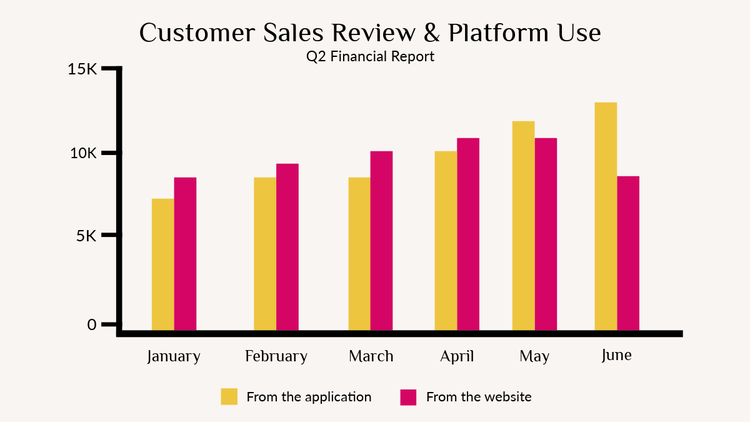
\includegraphics[width=5cm, height=3cm]{images/ejemplo.png}
    \caption{Envejecimiento en Europa}
    \label{fig:envejecimiento}
\end{figure}


\begin{table}[htbp]
    \centering
    \begin{tabular}{|c|c|c|}
        \hline
        \textbf{Nombre} & \textbf{Edad} & \textbf{Género} \\
        \hline
        Juan & 25 & Masculino \\
        María & 30 & Femenino \\
        Carlos & 22 & Masculino \\
        Ana & 28 & Femenino \\
        \hline
    \end{tabular}
    \caption{Ejemplo de tabla}
    \label{tab:ejemplo}
\end{table}
\newpage
¿Qué pasa si sigo escribiendo aquí? En principio debería poner en el encabezado la sección en la que estamos, pero no estoy seguro. Al parecer, funciona perfecto.

\newpage\printbibliography
\addcontentsline{toc}{section}{Referencias}
\end{document}
